\documentclass[10pt]{beamer}

%STANDARD PREAMBLE
%https://tex.stackexchange.com/questions/68821/is-it-possible-to-create-a-latex-preamble-header
\usepackage{/Users/miw267/Repos/latex_preamble/beamer_preamble}
%\usepackage{/Users/miw267/Repos/csci246_spring2025/slides/preambles/beamer_preamble_for_CSCI246}


%%%
% SPECIFIC TO THIS DOCUMENT 
%%%
\let\warning\relax
\usepackage{fourier} % has warning  and danger symbols. However, it makes the bottoms tuff bold. 

\renewcommand{\ELBO}{\texttt{ELBO}}
\renewcommand{\Q}{\mathcal{Q}}


%%%%
% DOCUMENT 
%%%
\title{04/07/2026: Denoising Diffusion Probabilistic Models}
\author{Reference: Ho, J., Jain, A., \& Abbeel, P. (2020). \textit{Denoising diffusion probabilistic models.}}
\date{CSCI 546: Diffusion Models}

\begin{document}
\maketitle

%\begin{frame}{Table of contents}
%  \setbeamertemplate{section in toc}[sections numbered]
%  \tableofcontents[hideallsubsections]
%\end{frame}

\begin{frame}{Table of contents}
  \setbeamertemplate{section in toc}[sections numbered]
  \setbeamertemplate{subsection in toc}[subsections numbered]
  \tableofcontents
\end{frame}





\section{Course Logistics}





\begin{frame}{A note on score matching}

Let 
\begin{itemize}
	\item $ p_0(\+x)$ be the density of the true data generating distribution
	\item $ p_\+\theta(\+x)$ be the density of our model.
\end{itemize}
\vfill 
\pause 
Then the \textbf{score matching} training loss is given by
\[ J(\+\theta) = \int \half \; || \labeledgreenmathbox{model score}{\nabla_\+x  \ln p_\+\theta(\+x)} -  \labeledredmathbox{true score}{\nabla_\+x  \ln p_0(\+x)}||^2 \;  p_0(\+x) \, d\+x\]
\vfill 
\pause 
\begin{myredbox}[title=Grading of Reading Survey \#5]
\begin{itemize}
	\item Many people gave mostly beautiful answers, but didn't mention the key contribution of the paper: how to get around the fact that the \textbf{true score} is unknown.  \pause 
	\item If you didn't mention this, but your answer was otherwise solid, you scored 3.5/4 =87\% (B+).
\end{itemize}

\end{myredbox}
\end{frame}


\begin{frame}{Reading Survey \#6}

\begin{enumerate}
	\item Relate today's paper to what we've learned earlier in the course.
\end{enumerate}
	
\end{frame}


\section{Lightning Chat}

\begin{frame}[standout]
\href{https://docs.google.com/presentation/d/137z9x9Dezg3Uj54vjpxikanr_5CEVu4gCx5uTogo6r8/edit?usp=sharing}{\alert{\underline{Lightning Chat}}}
\end{frame}



\section{Mini-Lecture}


\begin{frame}{Warmup: Diffusion Interpolations}


\colorbox{yellow!30}{\textbf{Poll.}} Who can explain what's going on in this picture? 

\begin{figure} 
\includegraphics[width=\textwidth]{images/interpolations} 
\end{figure}
	
\end{frame}

\begin{frame}

\colorbox{yellow!30}{\textbf{Poll.}} What is the takeaway?

\begin{figure} 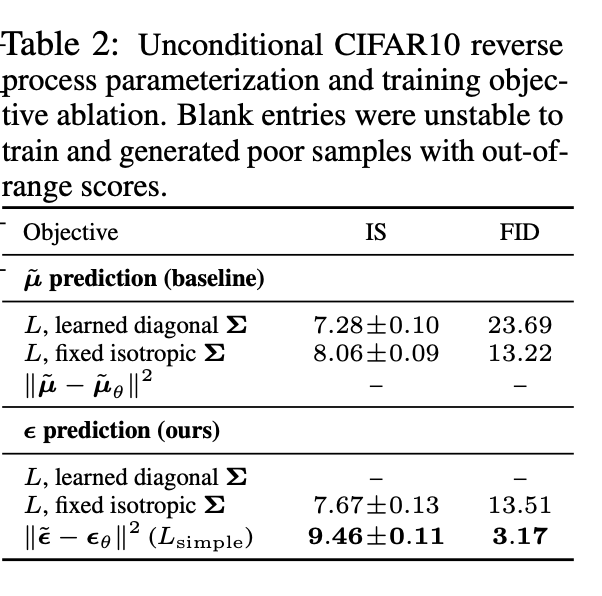
\includegraphics[width=.6\textwidth]{images/predicting_the_noise_results} 
\end{figure}

\pause 
\colorbox{green!30}{\textbf{Solution.}} Using the \qq{predicting the noise} training strategy \alert{hugely} improves the quality of generated samples.

\vfill 
\pause 
\colorbox{blue!30}{\textbf{Remark.}} This is consistent with the results of our coding workshop.

\end{frame}


\begin{frame}{Standard Approach: Predicting The (One-Step) Denoised Data}
\small 
\only<1->{
Ideally, we'd try find the weights $\+w$ of our neural network which maximize the likelihood of our data $\+x$
\[ p(\+x \mid \+w) = \int \cdots \int p(\+x, \+z_1, \hdots, \+z_T \mid \+w) \; \text{d}\+z_1 \hdots \text{d}\+z_T\]
}
%
\only<2->{
However, the exact integral is \alert{intractable}, because the integrals involve integrating over complex neural networks. 
}
%
\only<3->{
Instead, we do \textbf{variational inference}, finding the weights that maximize the \textit{evidence lower bound} (ELBO).
\[ p(\+x \mid \+w) \geq \ELBO(\+w),\]
}
%
\only<4-5>{
where
\begin{align*}
\ELBO(\+w) &=   \labeledgreenmathbox{reconstruction term}{\int q(\+z_1 \mid \+x) \ln p(\+x \mid \+z_1, \+w) \text{d} \+z_1} \\
& \quad 	- \labeledredmathbox{consistency terms}{\ds\sum_{t=2}^T \int \KL{q(\+z_{t-1} \mid \+z_t, \+x)}{p(\+z_{t-1} \mid \+z_t, \+w)} \, q(\+z_t \mid \+x )\text{d} \+z_t}
\end{align*}
}

\only<5>{
\colorbox{yellow!30}{\textbf{Poll.}} How can we simplify the ELBO into one line?
}

\only<6->{
where by defining $\+z_0 := \+x$, we have 
\begin{align*}
\ELBO(\+w) &=  \labeledredmathbox{one-step denoising terms}{- \ds\sum_{t=1}^T \int \KL{q(\+z_{t-1} \mid \+z_t, \+x)}{p(\+z_{t-1} \mid \+z_t, \+w)} \, q(\+z_t \mid \+x )\text{d} \+z_t}
\end{align*}
}
\end{frame}

\begin{frame}{Standard Approach: Predicting The (One-Step) Denoised Data}

\small

\only<1>{
\colorbox{yellow!30}{\textbf{Poll.}}  Our objective is to minimize $\KL{q(\+z_{t-1} \mid \+z_t, \+x)}{p(\+z_{t-1} \mid \+z_t, \+w)}$.  What is this term doing?  
}

\only<2->{
\colorbox{green!30}{\textbf{Solution.}} KL divergence is a measure of statistical distance.  So we're trying to minimize
\[\KL{ \labeledgreenmathbox{true denoising}{q(\+z_{t-1} \mid \+z_t, \+x)}}{\labeledredmathbox{approximate denoising}{p(\+z_{t-1} \mid \+z_t, \+w)}} \]
}


\only<3>{
\colorbox{yellow!30}{\textbf{Poll.}} What does each term represent concretely?
}

\only<4->{
By reversing the noising Markov chain, we can compute
\begin{align*}
\labeledgreenmathbox{true denoising}{q(\+z_{t-1} \mid \+z_t, \+x)} &= \N \bigg(\+m_t(\+z_t, \+x) \; , \; \sigma^2_t \+I \bigg),
\intertext{where}
\+m_t(\+z_t, \+x) &= \frac{(1-\alpha_{t-1}) \sqrt{1-\beta_t} \+z_t \; + \; \sqrt{\alpha_{t-1}} \beta_t \+x}{1-\alpha_t} \\
\sigma^2_t &= \frac{\beta_t (1-\alpha_{t-1})}{1-\alpha_t}
\end{align*}
}


\only<5->{
But this depends on $\+x$. So we try to match it with
%
\begin{align*}
\labeledredmathbox{approximate denoising}{p(\+z_{t-1} \mid \+z_t, \+w)} &= \N \bigg(\widehat{\+m}_t(\+z_t, \+w) \; , \; \sigma^2_t \+I \bigg).
\end{align*}

}

\end{frame}



\begin{frame}{Standard Approach: Predicting The (One-Step) Denoised Data}

Since the KL divergence 
\[\KL{ \labeledgreenmathbox{true denoising}{q(\+z_{t-1} \mid \+z_t, \+x)}}{\labeledredmathbox{approximate denoising}{p(\+z_{t-1} \mid \+z_t, \+w)}} \]
is between two Gaussians, it reduces to :

\begin{align*}
\frac{1}{2\beta_t} \; \norm{\labeledgreenmathbox{true denoising mean}{\+m_t(\+z_t, \+x)}  -  \labeledredmathbox{approximate denoising mean}{\widehat{\+m}_t(\+z_t, \+w)}}^2 \; + \; \texttt{const}
\end{align*}


\pause 
\colorbox{blue!30}{\textbf{Remark.}} Recall that our objective is to minimize the above summed over $t=1,..,T$. This reveals even more concretely that our objective is to \alert{predict one-step denoised data.}

\end{frame}



\begin{frame}{Proposed Approach: Predicting the noise}

Our paper proposes that instead our neural networks should learn to \alert{predict the noise}:

\begin{figure} 
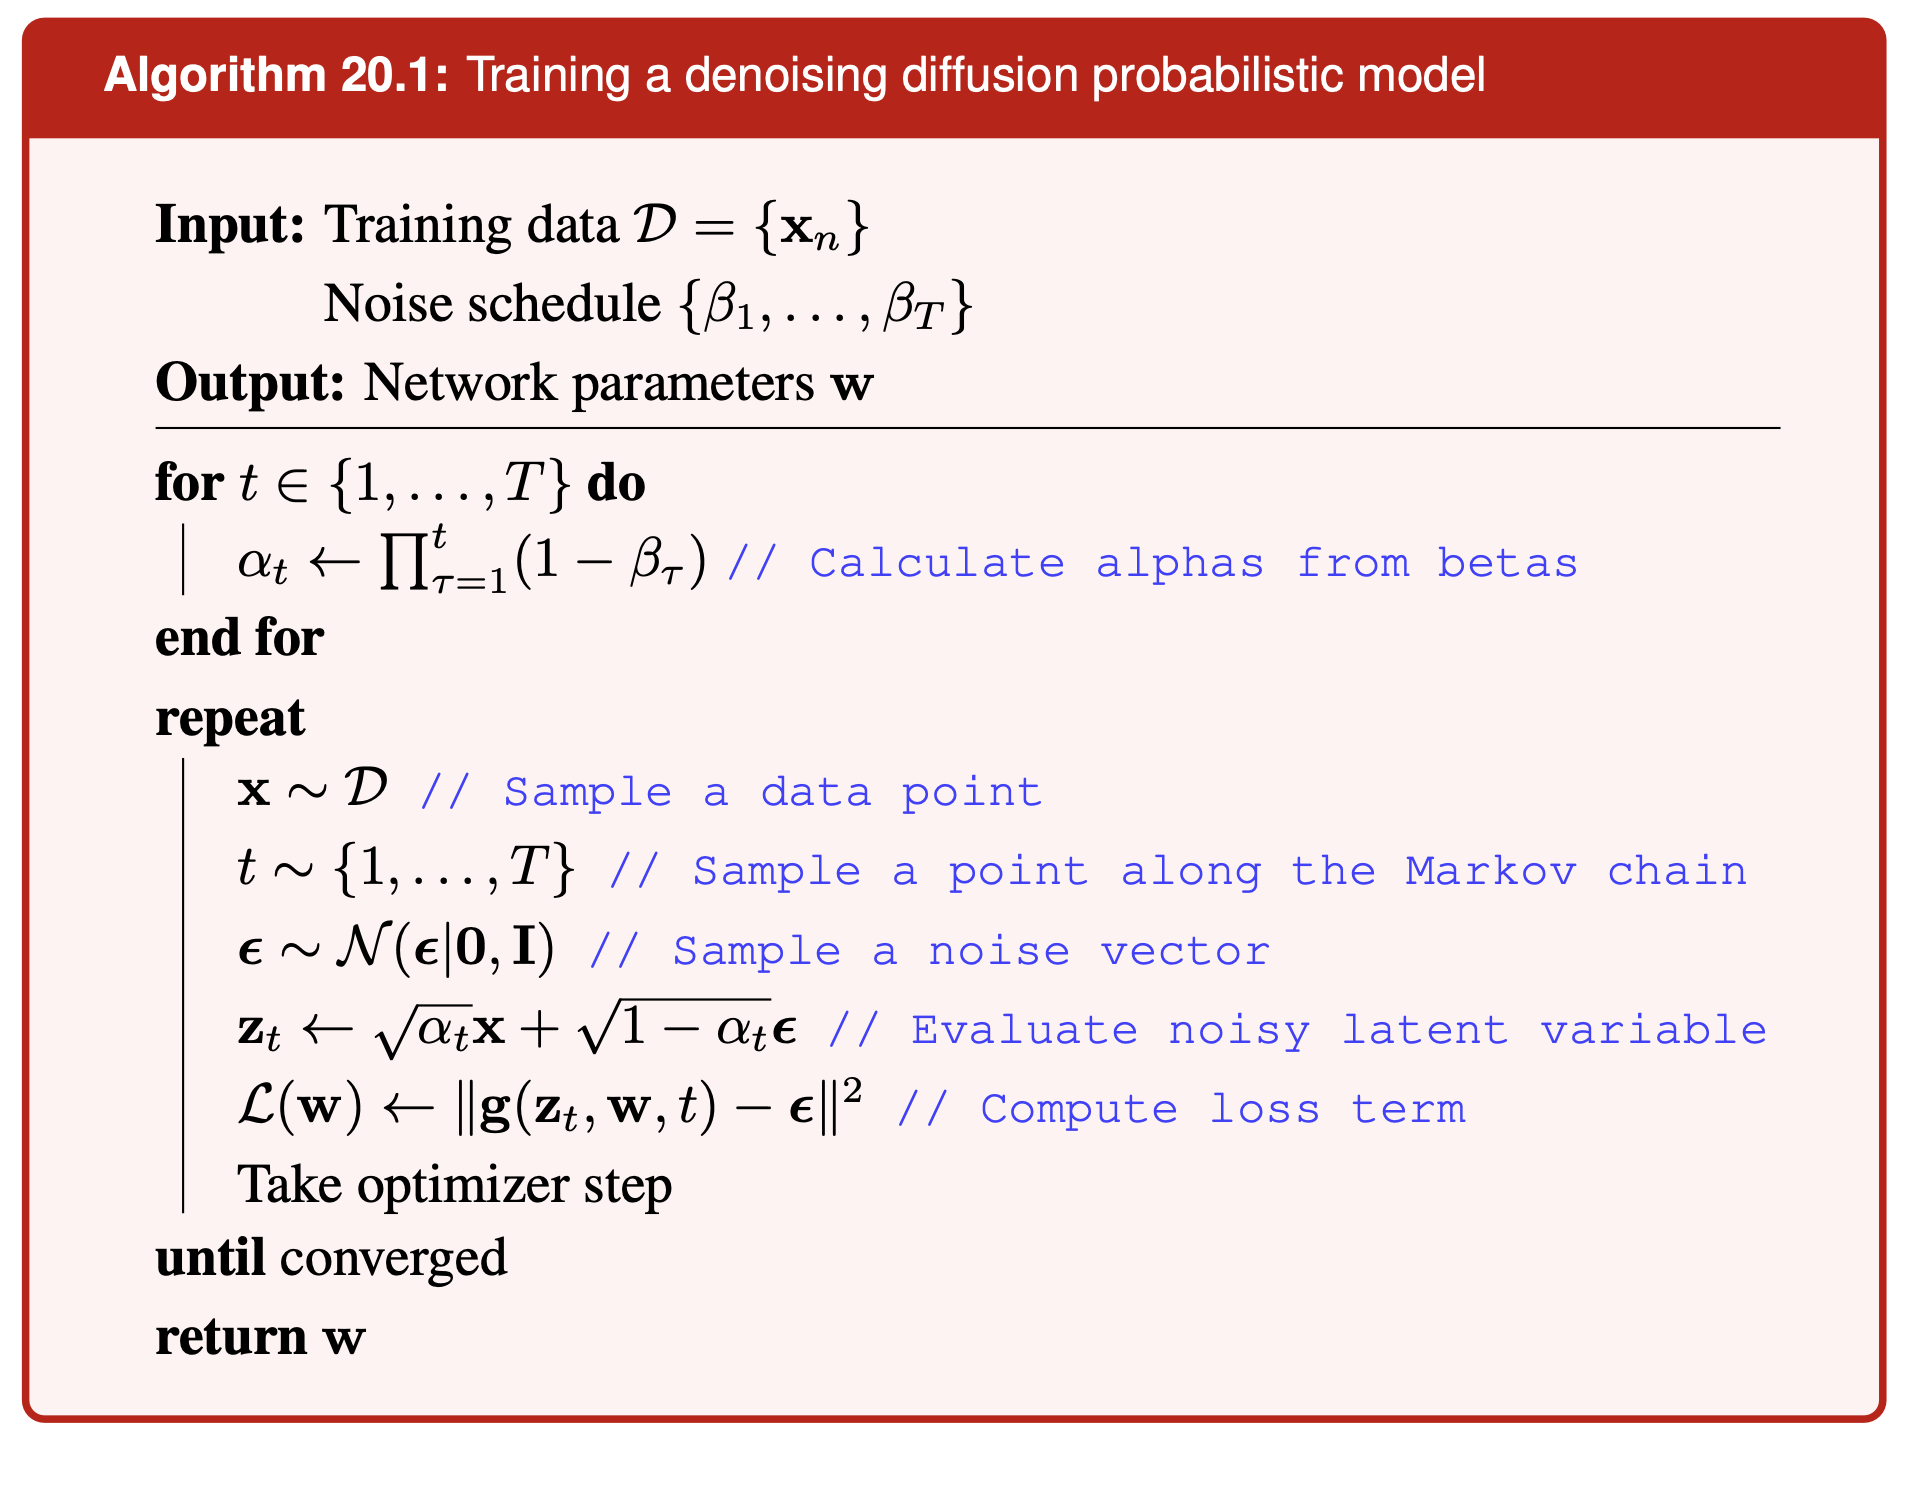
\includegraphics[width=.9\textwidth]{images/predicting_the_noise_algorithm} 
\end{figure}

\end{frame}


\section{Group Exercises}

\begin{frame}{Group exercise} 
\colorbox{blue!30}{\textbf{Exercise.}} Prove that the true denoised mean can be written as 
\[ \+m_t(\+z_t,\+x) = \frac{1}{\sqrt{1-\beta_t}} \bigg\{ \+z_t - \frac{\beta_t}{\sqrt{1-\alpha_t}} \+\epsilon_t \bigg\}. \]
When the approximate denoised mean $\widehat{\+m}_t(\+z_t,\+w)$ takes the same form but with $\widehat{\+\epsilon}_t(\+z_t, \+w)$,  this leads to the \qq{predicting the noise} formulation. %(Bishop pp. 591).
\pause 

\colorbox{green!30}{\textbf{Reference.}} 


\begin{align*}
\explaintermbrace{true denoising}{q(\+z_{t-1} \mid \+z_t, \+x)} &= \N \bigg(\+m_t(\+z_t, \+x) \; , \; \sigma^2_t \+I \bigg),
\intertext{\qquad where}
\+m_t(\+z_t, \+x) &= \frac{(1-\alpha_{t-1}) \sqrt{1-\beta_t} \+z_t \; + \; \sqrt{\alpha_{t-1}} \beta_t \+x}{1-\alpha_t} %\\
%\sigma^2_t &= \frac{\beta_t (1-\alpha_{t-1})}{1-\alpha_t}
\end{align*}


\begin{align*}
\explaintermbrace{multi-step noising}{q(\+z_t \mid \+x)} = \N \bigg(\sqrt{\alpha_t} \+x \; , (1-\alpha_t) \+I \bigg), \qquad \text{where} \quad  \alpha_t = \prod_{s=1}^t (1-\beta_s)
\end{align*}

\end{frame}






\end{document}

